\subsection{APLICACIÓN DEL MÉTODO DE VALOR AGREGADO ESTIMADO (EVA).}\label{5.2}

\subsubsection{Estimación del Costo de Capital conforme al modelo CAPM. }

\begin{figure}
\centering
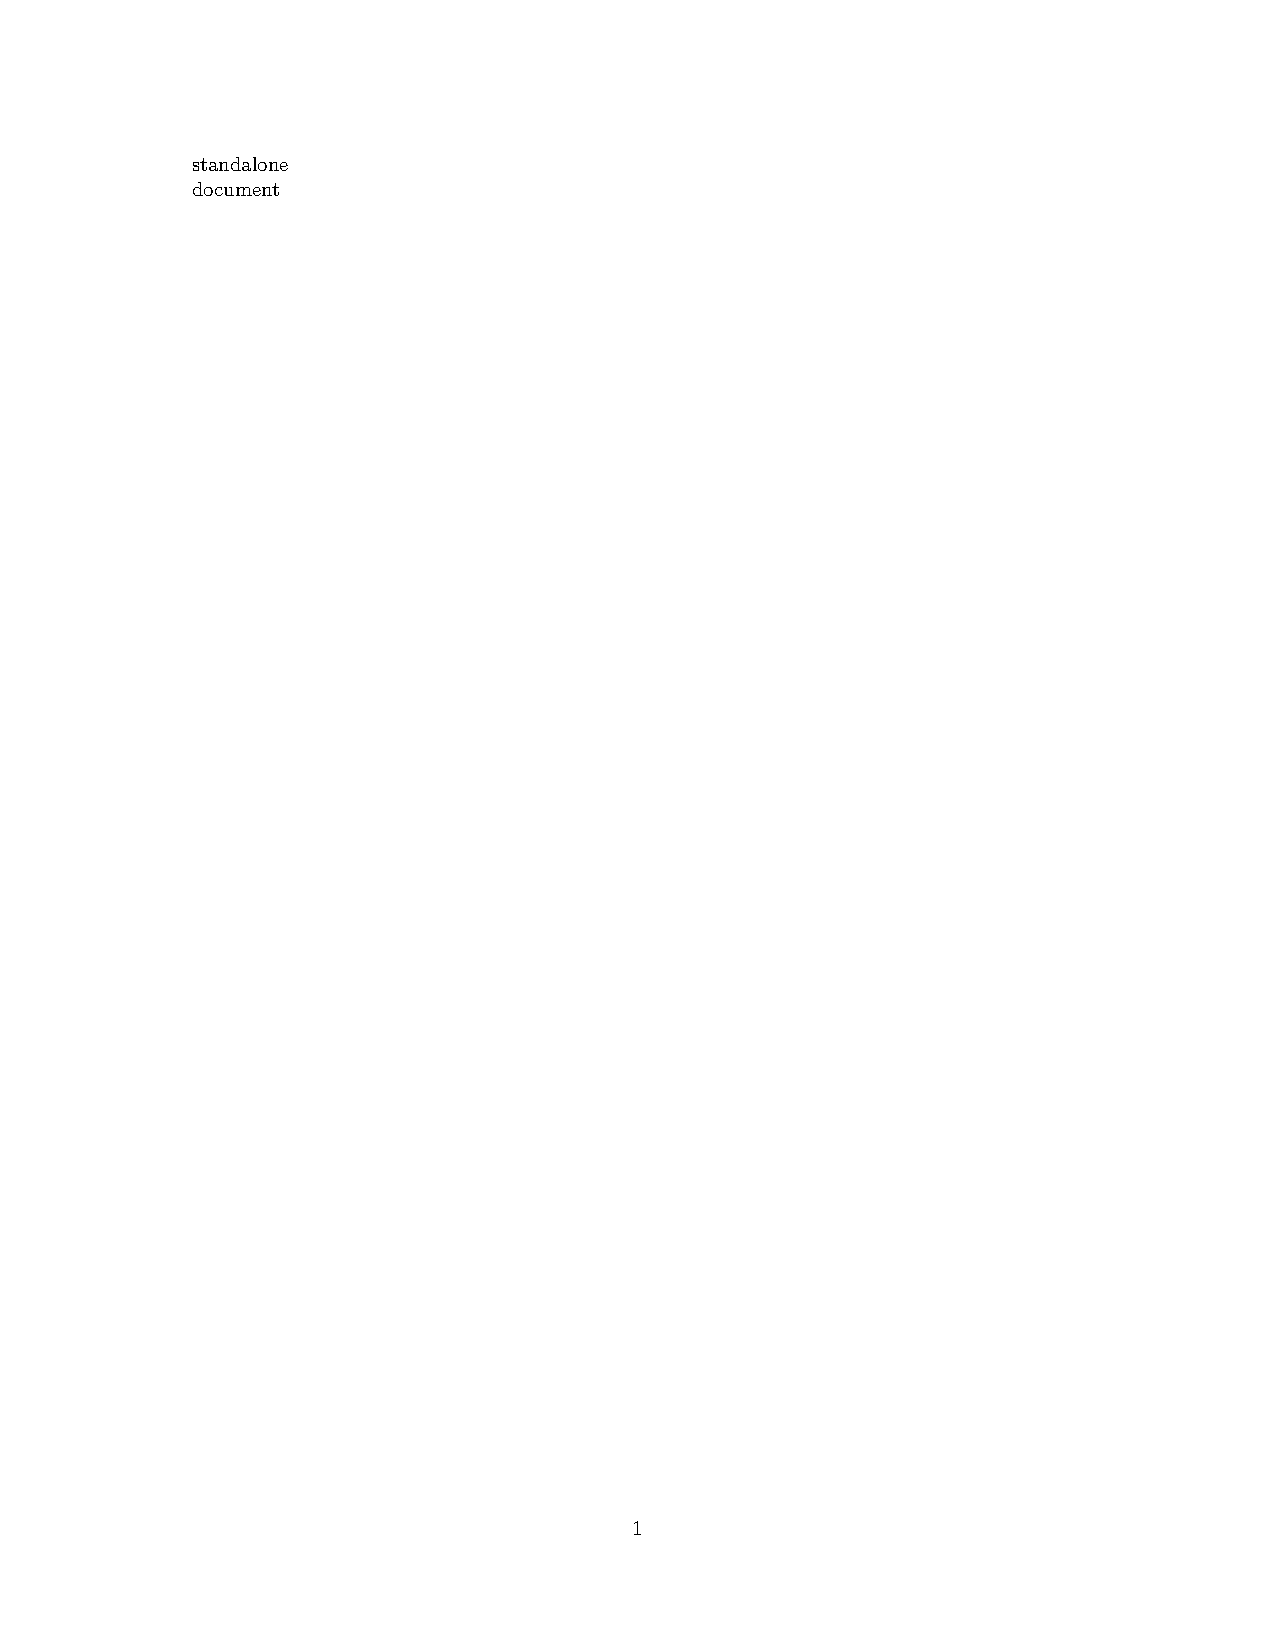
\includegraphics[width=10cm]{\rutaImagenes/wacc_wara}
\end{figure}

\textcolor{principal}{Tasa de descuento para activos intangibles}.- La tasa de descuento generalmente aplicable a la estimación de activos intangibles puede cuantificarse con los modelos financieros conocidos como WACC y/o WARA, entre otros:\\

\textcolor{principal}{WACC (costo promedio ponderado de capital)}. El costo de capital es la compensación que los inversionistas exigen de parte de las firmas que utilizan sus fondos (costo de oportunidad). \\

\textcolor{principal}{MODELO DE VALORACIÓN DE ACTIVOS DE CAPITAL (CAPM)}. El CAPM establece que los accionistas deben de ganar por su inversión al menos una tasa libre de riesgo, más un diferencial que compense el premio del mercado por el riesgo sistemático de dicha inversión. 

\begin{figure}
\centering
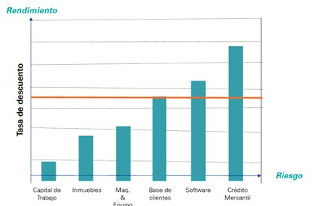
\includegraphics[width=8cm]{\rutaImagenes/costo_oportunidad_accionistas}
\end{figure}

Cuanto mayor sea el riesgo sistemático de una acción, más elevado será el rendimiento que los inversionistas esperarán de sus activos.  

\begin{enumerate}[a)]
\item Costo de Capital (para accionistas diversificados):\\

\begin{center}
\begin{minipage}{8cm}
\begin{itemize}
\small
				\item El costo del capital accionario se estima utilizando el \textit{Capital Asset Pricing Model} (\gls{capm}):
				$$Rk=Rf+\beta\times(ERP)$$
				 \item Donde:
				 \item $Rf$= Tasa Libre de Riesgo
				 \item $ERP$= Prima de Riesgo del Mercado de Capitales
				 \item $\beta$=\gls{beta}
			\end{itemize}
	\footnotesize{Fuente: Valuaci\'on de Activos Intangibles. DEAL ADVISORY MEXICO. KPMG C\'ARDENAS DOSAL, S.C. KPMG ``D.R.''\copyright 2016.}
		\end{minipage}
\end{center}


El resultado del costo de capital (KE) como tasa mínima de retorno aceptable para activos fondeados por capital accionario, con un resultado de 14.38\% (ke).\\

\begin{figure}
\centering
\includegraphics[width=8cm]{../0.imagenes/ke}
\end{figure}

Se agregan los generadores así como la evidencia del muestreo de banca de inversión al APÉNDICE 6.

\item Costo de la deuda:\\

\begin{figure}
\centering
\includegraphics[width=8cm]{../0.imagenes/kd}
\end{figure}

El resultado del costo de fondeo de la deuda antes de impuestos (Kd) es de 13.19\%.

\item Estimación de la WACC:\\

Consiste en la tasa a la cual son descontados todos los proyectos de la entidad. Se dice que la rentabilidad mínima producto de su operación debiera ser la WACC, ya que considera en su cálculo la proporción de deuda explícita y capital propio, beneficio fiscal a la deuda, así como la intervención de las tasas Kd y Ke, dada la mezcla de capitales en inversión. Se utilizó la fórmula que se muestra a continuación:\\

$$WACC=\left(kd(1-t)\fracc{D}{D+E}\right)+\left(ke\fracc{E}{D+E}\right)$$

De esta manera, el resultado del Costo promedio ponderado de capital en Pesos (MXN) es de: 11.73\%.

 \begin{figure}
\centering
\includegraphics[width=8cm]{../0.imagenes/wacc}
\end{figure}

\end{enumerate}

\subsubsection{Estimación del Deterioro y el Lucro Cesante por Producto correspondiente a la marca, por el método EVA conforme al modelo \ref{5.2}:}

\begin{figure}
\centering
\includegraphics[width=\textwidth]{../0.imagenes/eva_1}
\end{figure}

\begin{figure}
\centering
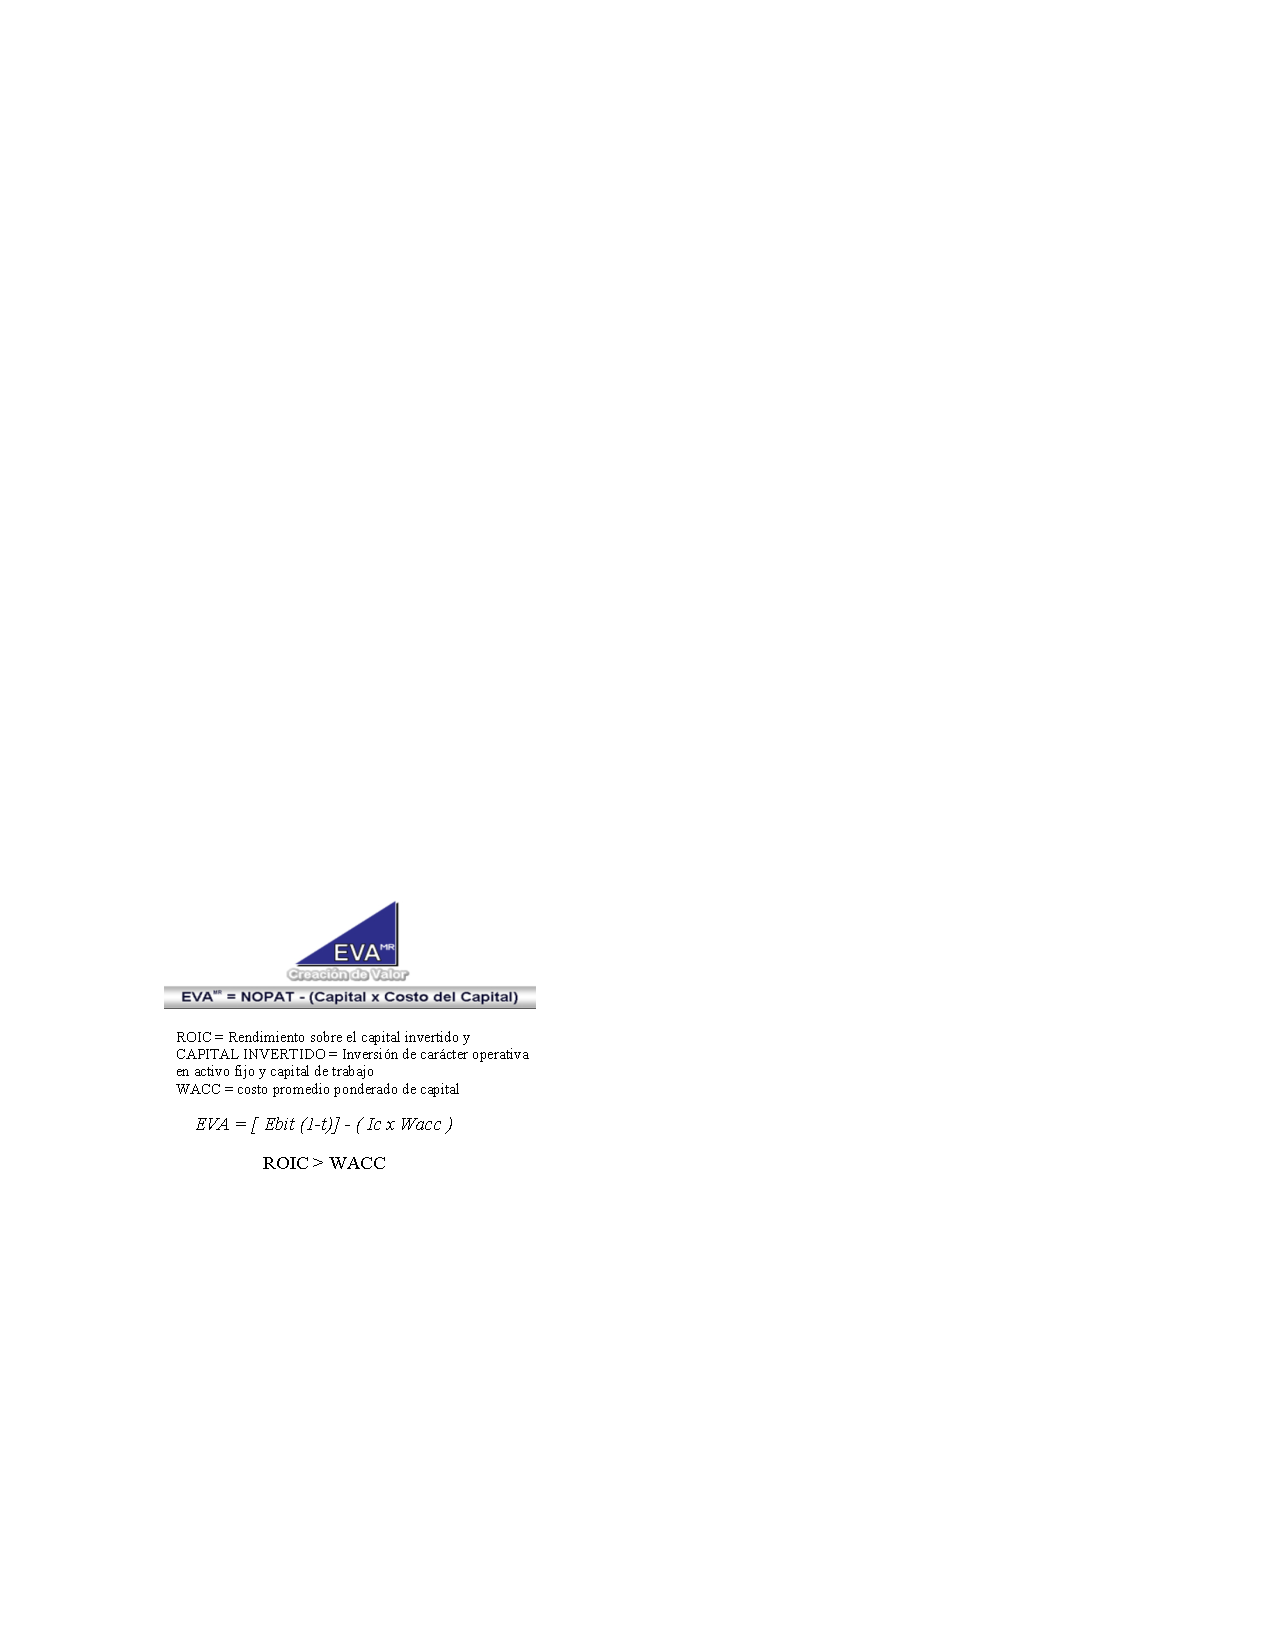
\includegraphics[width=\textwidth]{../0.imagenes/eva_2}
\end{figure}

\begin{figure}
\centering
\includegraphics[width=.7\textwidth]{../0.imagenes/eva_3}
\end{figure}

